
% O \emph{Astrobees} é um sistema robótico desenvolvido pela NASA para operar na ISS, conforme \cite{nasaAstrobee} explica, este dispositivo auxilia os astronautas em tarefas rotineiras e também para explorar novas tecnologias de robótica em microgravidade. Ao todo são três robôs autônomos denominados como \emph{Honey}, \emph{Bumble} e \emph{Queen}. O \emph{Astrobee} é um cubo de 31,75 cm de cada lado, e pode funcionar de forma autônoma ou ser controlado remotamente, variando conforme as necessidades da missão. Eles são capazes de realizar inspeções, monitorar equipamentos, documentar experimentos e transportar pequenos objetos dentro da ISS. Essas ações permitem que os astronautas concentrem seu tempo em atividades mais críticas como as pesquisas a serem desenvolvidas e na manutenção da ISS.

Os \emph{Astrobees} são equipados com sensores e câmeras, além disso, tecnologias avançadas de navegação com visão computacional são usadas para se mover com precisão no ambiente de microgravidade da estação espacial.
% O sistema é alimentado por propulsores de ventilador que permitem sua movimentação em todas as direções e ele é capaz de retornar de forma autônoma à sua estação de recarga, o que permite operação contínua e sem intervenção humana direta. Essa capacidade autônoma é suportada por algoritmos de aprendizado de máquina que aprimoram sua eficiência ao longo do tempo \cite{nasaAstrobee}.
Este sistema robótico é capaz de retornar de forma autônoma à sua estação de recarga, permitindo operação contínua e sem intervenção humana direta. 
Essa capacidade autônoma é suportada por algoritmos de aprendizado de máquina que aprimoram o seu trabalho ao longo do tempo \cite{nasaAstrobee}.

\begin{figure}[H]
    \centering
    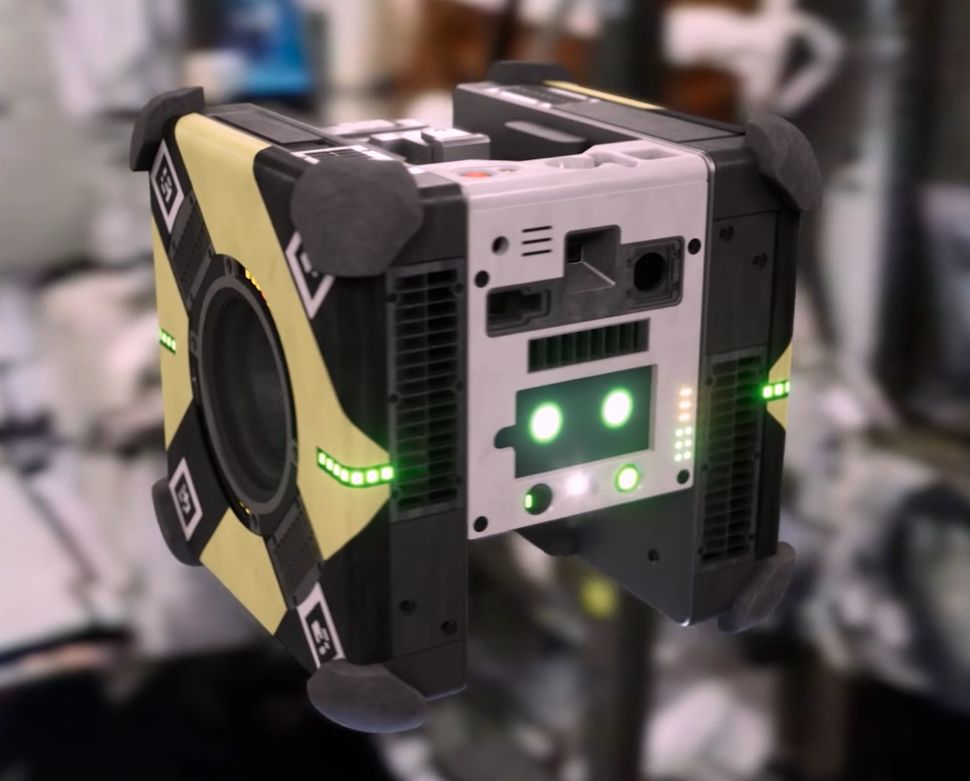
\includegraphics[width=1\linewidth]{1 Introducao/Imagens/Astrobee NASA.png}
    \caption{Astrobee, robô auxiliar dos pesquisadores na ISS. Fonte: Space.com (https://www.space.com/astrobee-robots-on-space-station.html).}
    \label{fig:AstrobeeFoto}
\end{figure}

% Adicionalmente, os \emph{Astrobees} servem como uma plataforma de teste para novas tecnologias espaciais. Os pesquisadores podem carregar e testar software personalizado nos robôs para simular cenários de futuras missões espaciais para desenvolver soluções para operações em estações espaciais futuras como o \emph{Lunar Gateway}, que será utilizada em missões no espaço profundo \cite{nasaAstrobee}.
